\documentclass[a4paper,10pt]{article}
\usepackage[utf8x]{inputenc}
\usepackage{verbatim}
\usepackage{graphicx}

%opening
\title{Lab 3}
\author{William Richard}

\begin{document}

\maketitle

\section{sudo}
\subsection{Text Answers}
\begin{verbatim}
Try running a root command from your shell.
What happened? 
You need to be root to perform this command.

The Plan:

I) /etc/sudoers.original
II) User_Alias FULLTIMERS = wrichard,jerry
III) Cmnd_Alias SHUTDOWN = /sbin/shutdown
IV) Host_Alias HOSTS = localhost.localdomain
V) Defaults:FULLTIMERS    !lecture
VI) wrichard ALL = (ALL) ALL
VII) cat ALL = SHUTDOWN
VIII) wrichard HOSTS = (ALL) ALL
      tom HOSTS = (ALL) ALL
\end{verbatim}
\subsection{The Execution}
1. 
\begin{center}
 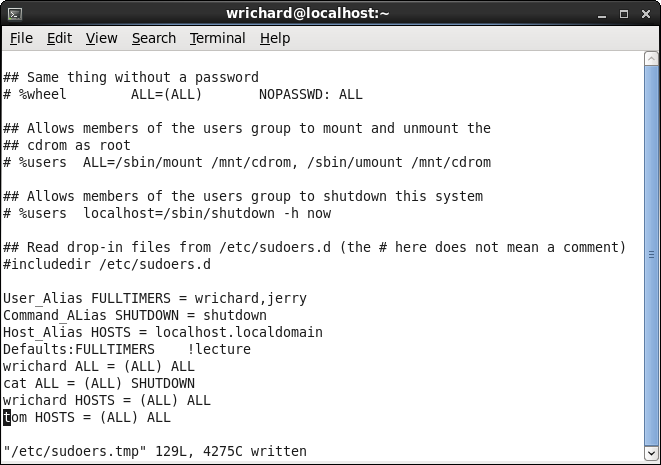
\includegraphics[width=\linewidth]{./sudoersfile.png}
\end{center}
c.
\begin{center}
 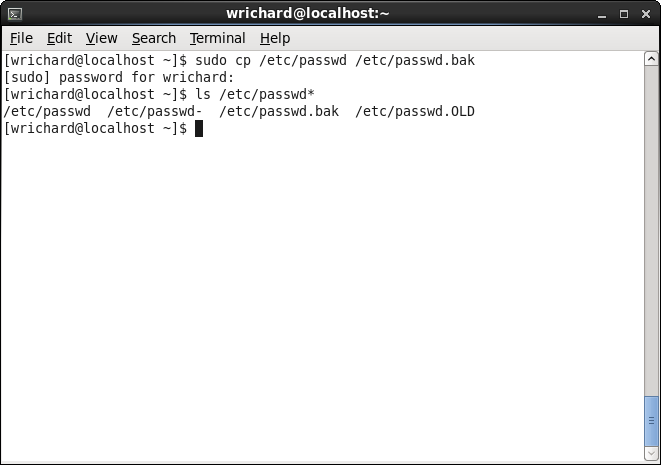
\includegraphics[width=\linewidth]{./passwd.png}
\end{center}

\section{Users and Groups}
\subsection{Spikes home}
\begin{center}
 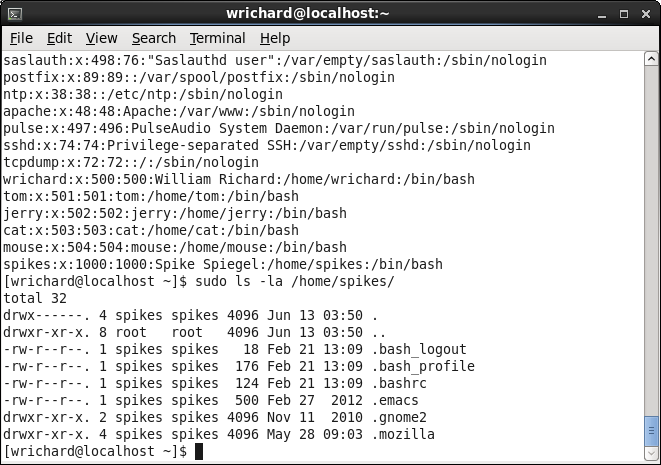
\includegraphics[width=\linewidth]{./spikeshome.png}
\end{center}

\subsection{Spikes password}
\begin{center}
 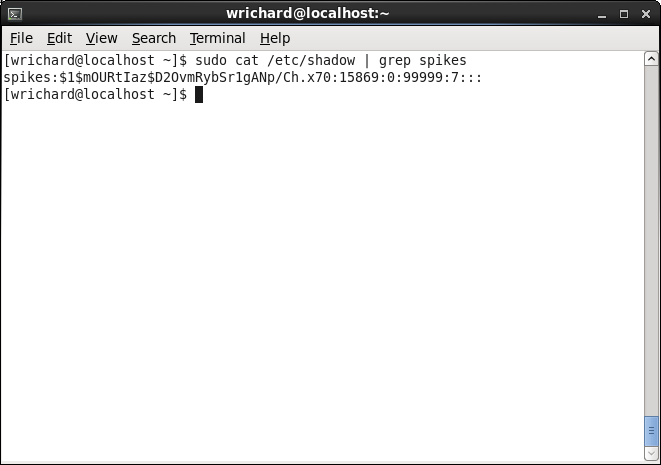
\includegraphics[width=\linewidth]{./spikespasswd.png}
\end{center}

\subsection{Spikes terminal}
\begin{center}
 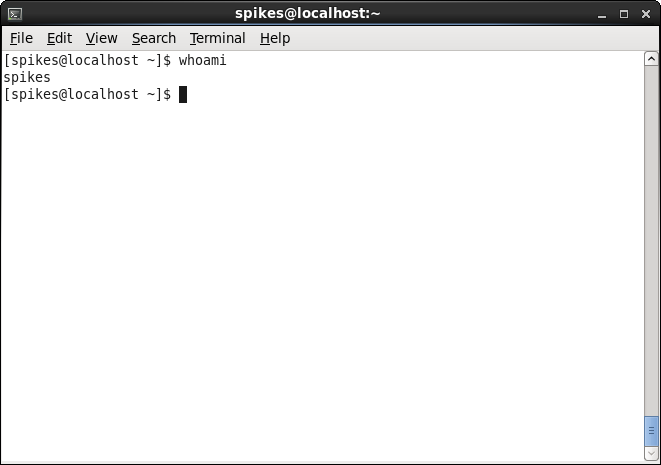
\includegraphics[width=\linewidth]{./spikesterminal.png}
\end{center}

\subsection{Add new users}

\verbatiminput{add_new_users.sh}

\begin{center}
 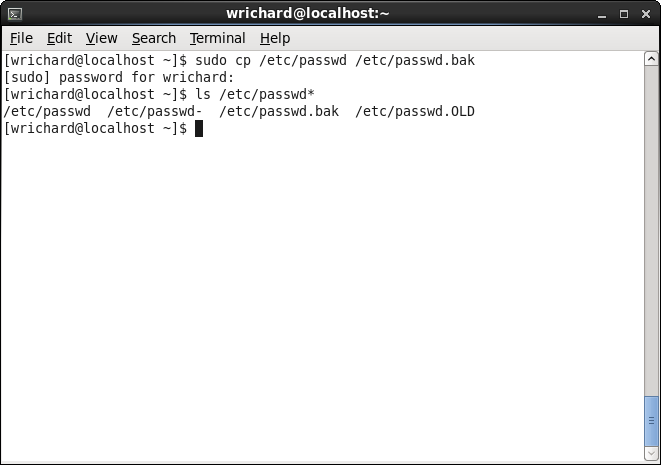
\includegraphics[width=\linewidth]{./passwd.png}
\end{center}



\end{document}
